\documentclass{standalone}
\usepackage{tikz,pgfplots}
\begin{document}
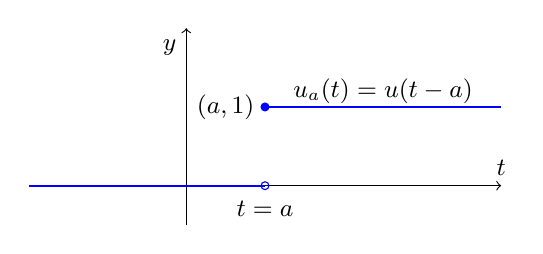
\begin{tikzpicture}[font=\small]
\coordinate (1) at (1, 0);
\coordinate (2) at (1, 1);
\draw [->] (-2, 0) -- (4, 0) node [pos=1, above] {$t$};
\draw [->] (0, -0.5) -- (0, 2) node [pos=0.9, left] {$y$};
\draw [blue,thick] (-2, 0) -- (1, 0);
\draw [blue,thick] (1, 1) -- (4, 1);
\draw [blue] (1) circle (0.05);
\draw [fill, blue] (2) circle (0.05);
\draw (1, -0.3) node {$t=a$};
\draw (0.5, 1) node {$(a,1)$};
\draw (2.5, 1.2) node {$u_{a}(t) = u(t-a)$};
\end{tikzpicture}
\end{document}